\documentclass[twoside]{../zirkelblatt1415}
\usepackage{mathtools}
\let\raggedsection\centering

\theoremstyle{definition}
\newtheorem{defn}{Definition}[section]
\newtheorem{defn'}{Vorläufge Definition}[section]
\newtheorem{axiom}[defn]{Axiom}
\newtheorem{bsp}[defn]{Beispiel}

\theoremstyle{plain}

\newtheorem{prop}[defn]{Proposition}
\newtheorem{motto}[defn]{Motto}
\newtheorem{wunder}[defn]{Wunder}
\newtheorem{ueberlegung}[defn]{Überlegung}
\newtheorem{lemma}[defn]{Lemma}
\newtheorem{kor}[defn]{Korollar}
\newtheorem{hilfsaussage}[defn]{Hilfsaussage}
\newtheorem{satz}[defn]{Satz}
\newtheorem{thm}[defn]{Theorem}

\theoremstyle{remark}
\newtheorem{bem}[defn]{Bemerkung}
\newtheorem{warnung}[defn]{Warnung}
\newtheorem{aufg}[defn]{Aufgabe}

\definecolor{darkred}{rgb}{0.7,0,0}
\definecolor{shadecolor}{rgb}{.95,.95,.95}

\newcommand{\defeq}{\vcentcolon=}

\DeclareMathOperator{\ld}{ld}
\newcommand{\RR}{\mathbb{R}}
\newcommand{\CC}{\mathbb{C}}
\newcommand{\Res}{\mathrm{Res}}

\usepackage[T1]{fontenc}
\usepackage{libertine}

\begin{document}

\maketitleCustom{Klassen 10/11/12}{\textbf{\textsf{%
  Der Residuensatz \\
  \normalsize Zirkelzettel vom 20. März 2015}}}

{\renewcommand{\addvspace}[1]{\vskip0.6em}
\tableofcontents%
}


\section{Das komplexe Kurvenintegral}

In der Schule integriert man Funktionen~$f : \RR \to \RR$ längs Intervallen,
also gewissen Ausschnitten der reellen Zahlengerade. Man schreibt dafür
\[ \int_a^b f(x) \,dx \qquad\text{oder}\qquad \int\limits_{[a,b]} f(x) \,dx. \]
Wir möchten nun Funktionen~$f : \CC \to \CC$ längs \emph{Kurven in der
komplexen Zahlenebene} integrieren. Die Werte solcher Funktionen sind also
komplexe Zahlen, die von einem komplexen (statt reellen) Parameter abhängen.
Ist~$L$ eine solche Kurve, so schreiben wir \[ \int_L f(z) \,dz \] für das
Integral von~$f$ längs~$L$. Im Spezialfall, dass~$L$ \emph{geschlossen ist}
(also Anfangs- und Endpunkt von~$L$ übereinstimmen), so schreiben wir zur
Betonung gelegentlich \[ \oint_L f(z) \,dz. \]

Wie berechnet man ein solches Integral? Wie ist ein solches Integral überhaupt
definiert? Dafür verwendet man \emph{Parametrisierungen}. Eine Parametrisierung
einer Kurve~$L$ ist eine bijektive Abbildung~$\gamma : [a,b] \to \CC$, deren
Werte genau die Punkte von~$L$ ablaufen. Hat man eine solche Parametrisierung
gefunden, so definiert man
\[ \int_L f(z) \,dz \defeq \int_a^b f(\gamma(t)) \, \gamma'(t) \,dt. \]

\begin{bem}Ein und dieselbe Kurve~$L$ kann durch mehrere verschiedene
Abbildungen parametrisiert werden. Man kann zeigen, dass der Wert des
Kurvenintegrals aber bei jeder Parametrisierung der gleiche ist.\end{bem}

\begin{bem}Für die Ableitung~$\gamma'$ einer komplexwertigen Funktion~$\gamma$
gelten dieselben Rechenregeln wie für die aus der Schule bekannten
reellwertigen Funktionen. Zum Beispiel ist die Ableitung der Funktion~$\gamma$
mit~$\gamma(t) = 7t + i t^2$ die Funktion~$\gamma'$ mit~$\gamma'(t) = 7 + 2ti$.
Die Zahl~$i$ wird also einfach als Konstante betrachtet.
\end{bem}

\begin{aufgabe}{Beispiele für Parametrisierungen}
Welche Kurven werden durch die folgenden Abbildungen parametrisiert?
\begin{enumerate}
\item $\gamma : [0,1] \to \CC,\ t \mapsto 3+t.$
\item $\gamma : [0,2] \to \CC,\ t \mapsto t + i t^2.$
\item $\gamma : [0,2\pi] \to \CC,\ t \mapsto e^{it}.$
\end{enumerate}
\emph{Tipp für Teilaufgabe~c):} Es gilt~$e^{it} = \cos(t) + i \sin(t)$. Wo
liegt diese Zahl in der komplexen Zahlenebene?
\end{aufgabe}

\begin{aufgabe}{Parametrisierungen von Kreisen}
Finde eine Parametrisierung des \ldots
\begin{enumerate}
\item Einheitskreises (damit ist immer gemeint: entgegen des Uhrzeigersinns),
\item um den Faktor~$r$ vergrößerten Einheitskreises,
\item Kreises mit Radius~$r$ und Mittelpunkt~$p$.
\end{enumerate}
\fixlistspacing
\end{aufgabe}

\begin{aufgabe}{Die Mutter aller komplexen Kurvenintegrale}
Berechne das Integral von~$1/z$ längs des Einheitskreises.
\end{aufgabe}

\begin{aufgabe}{Weitere wichtige komplexe Kurvenintegrale}
Der Integrationsweg~$L$ sei in den folgenden Fällen stets der Einheitskreis.
\begin{enumerate}
\item Was ist~$\oint_L z \,dz$?
\item Was ist~$\oint_L z^2 \,dz$?
\item Was ist~$\oint_L \frac{1}{z^2} \,dz$?
\end{enumerate}
\end{aufgabe}

\begin{aufgabe}{Vergleich mit dem gewöhnlichen Integral}
Sei~$[a,b]$ ein Intervall auf der reellen Zahlengerade. Dieses können wir auch
als (ungekrümmte) Kurve~$L$ in der komplexen Zahlenebene auffassen. Was ist der
Zusammenhang zwischen dem altbekannten Integral~$\int_a^b$ und dem
Kurvenintegral~$\int_L$? Beweise deine Vermutung, indem du eine
Parametrisierung von~$L$ angibst und die Definition des Kurvenintegrals
verwendest!
\end{aufgabe}


\section{Die Laurentwicklung von komplexen Funktionen}

Eine \emph{Laurentreihe} mit Entwicklungspunkt~$c$ ist eine Reihe der Form
\[ \cdots + a_{-2} (z-c)^{-2} + a_{-1} (z-c)^{-1} + a_0 + a_1 (z-c) + a_2 (z-c)^2 + \cdots, \]
wobei die Koeffizienten~$a_n$ beliebige komplexe Zahlen sein können. Eine
Laurentreihe mit Entwicklungspunkt~$0$ ist also von der Form
\[ \cdots + a_{-2} z^{-2} + a_{-1} z^{-1} + a_0 + a_1 z + a_2 z^2 + \cdots. \]
Viele komplexe Funktionen lassen sich auf diese Form bringen.

\begin{bsp}Die Laurentreihe des Polynoms~$5 z^2 - 3z + 8$ mit
Entwicklungspunkt~$0$ lässt sich sofort ablesen: Die meisten Koeffizienten sind
Null. Die einzigen Ausnahmen sind~$a_0 = 8$, $a_1 = -3$ und~$a_2 = 5$.\end{bsp}

\begin{aufgabe}{Beispiele für Laurententwicklungen}
Finde jeweils eine Laurententwicklung mit Entwicklungspunkt~$0$ von \ldots
\begin{enumerate}
\item $\frac{1}{1 - z}$,
\item $\frac{1}{1 - z^2}$,
\item $e^{\frac{1}{z}}$,
\item $\frac{1}{(z - i) (z + i)}$.
\end{enumerate}
\emph{Tipp:} Verwende die Formel für die geometrische Reihe, $\sum_{n=0}^\infty
q^n = \frac{1}{1 - q}$. Für Teilaufgabe~c) ist die Identität~$e^z = 1 + z + z^2/2 +
z^3/3! + z^4/4! + \cdots$ nützlich.
\end{aufgabe}

Der Koeffizient~$a_{-1}$ ist besonders wichtig. Er heißt auch \emph{Residuum}
der Laurentreihe an dem gegebenen Entwicklungspunkt. Für die Integration längs
eines beliebig kleinen Kreises~$K$ um den Ursprung gilt nämlich
\[ \oint_K (\cdots + a_{-1} z^{-1} + \cdots) \,dz = 2\pi i \cdot a_{-1}. \]
All die anderen Koeffizienten spielen also keine Rolle!

\begin{aufgabe}{Baby-Version des Residuensatzes}\label{aufg:residuensatz-baby}
Beweise diese Formel.
\end{aufgabe}

Eine \emph{holomorphe Funktion} ist eine, in deren Laurententwicklungen (um
jeden Punkt) nur nichtnegative Exponenten vorkommen. Solche Funktionen sind
also \emph{überall definiert} und besitzen keine Polstellen. Unter anderem sind
folgende Funktionen holomorph:
\begin{itemize}
\item Jedes Polynom, zum Beispiel $5z^2 - 3z + 8$.
\item Die Exponentialfunktion.
\item Die Summe zweier holomorphen Funktionen.
\item Das Produkt zweier holomorphen Funktionen.
\item Die Verkettung zweier holomorphen Funktionen.
\end{itemize}
Der Quotient zweier holomorpher Funktionen hat im Allgemeinen Polstellen
-- nämlich dort, wo der Nenner Nullstellen hat. Solche Funktionen heißen
\emph{meromorph}. In deren Laurententwicklung dürfen endlich viele -- aber
nicht unendlich viele! -- negative Exponenten vorkommen. Zum Beispiel sind die
Funktionen
\[ \frac{1}{z} \qquad \frac{z^2 - 3}{z^2 - 1} \qquad \frac{1}{z^2 + 1} \]
meromorph. Die Funktion~$\frac{z^2 - 2z + 1}{z - 1}$ scheint ebenfalls nur
meromorph zu sein, tatsächlich aber ist sie holomorph (wieso?).

\begin{aufgabe}{Formeln fürs Residuum}\label{aufg:residuum-formeln}
\begin{enumerate}
\item Sei~$f$ eine holomorphe Funktion. Erkläre, wieso das Residuum von~$f$ an
jeder Stelle Null ist.
\item Sei~$f$ eine meromorphe Funktion, die an einem Punkt~$c$ eine
\emph{einfache Polstelle} besitzt. Das bedeutet, dass die Laurententwicklung
von~$f$ um~$c$ so aussieht:
\[ f(z) = a_{-1} (z-c)^{-1} + a_0 + a_1 (z-c) + a_2 (z-c)^2 + \cdots. \]
Zeige, dass das Residuum von~$f$ bei~$c$, also~$a_{-1}$, über folgende Formel
berechnet werden kann:
\[ a_{-1} = \lim_{z \to c} \bigl((z-c) f(z)\bigr). \]
\item Sei~$f$ eine meromorphe Funktion mit~$f(z) = g(z) / h(z)$. Sei~$h(c) = 0$
und~$h'(c) \neq 0$. (Somit besitzt~$f$ eine einfache Polstelle bei~$c$.) Zeige,
dass das Residuum von~$f$ bei~$c$ dann gleich~$g(c) / h'(c)$ ist.
\end{enumerate}\fixlistspacing
\end{aufgabe}


\section{Der Residuensatz}

Das tolle an holomorphen und meromorphen Funktionen ist, dass man bei der
Berechnung des Kurvenintegrals den Integrationsweg deformieren kann, ohne dass
sich der Integralwert ändert! Das ist etwas ganz besonderes, zu dem es auch
kein reelles Analogon gibt -- schließlich lassen sich Intervalle auf der
eindimensionalen reellen Zahlengerade auch gar nicht deformieren.

Eine präzisere Aussage lautet: Sei~$f$ eine meromorphe Funktion. Sei~$K$ eine
Kurve in der komplexen Zahlenebene. Lasse sich~$K$ zu einer anderen Kurve~$L$
deformieren, \emph{ohne dabei die Polstellen von~$f$ zu überstreichen}. Dann
ist~$\int_K f(z) \,dz = \int_L f(z) \,dz$.

Seien zum Beispiel die Pole von~$f$ wie durch die roten Punkte gekennzeichnet
verteilt. Dann spielt es keine Rolle, ob man über die blaue oder die rosa Kurve
der linken Skizze integriert. Es macht aber durchaus einen Unterschied, ob man
über die blaue oder die rosa Kurve der rechten Seite integriert. Denn bei
dieser Deformation hat man den oberen rechten Pol überstrichen.

\begin{center}
\includegraphics[scale=0.75]{path-independence-1}\qquad\qquad
\includegraphics[scale=0.75]{path-independence-2}
\end{center}

In der folgenden Aufgabe beweist du den mächtigen Residuensatz. Er erlaubt es,
auch Integrale mit komplizierten Integrationswegen ganz einfach zu berechnen.
\begin{aufgabe}{Der Residuensatz}
Sei~$f$ eine meromorphe Funktion. Sei~$K$ eine geschlossene Kurve in der
komplexen Zahlenebene, die alle Polstellen von~$f$ in ihrem Inneren umfasst.
Beweise: Das Integral~$\int_K f(z) \,dz$ ist gleich der Summe der Residuen
von~$f$ an den Polstellen, multipliziert mit~$2 \pi i$. Als Formel:
\[ \oint_K f(z) \,dz = \sum_z \Res(f,z) \cdot 2 \pi i. \]
Deformiere dazu den Integrationsweg auf geeignete Art und Weise und verwende
Aufgabe~\ref{aufg:residuensatz-baby}. Verwende außerdem folgende Rechenregeln:
Setzt sich eine Kurve aus mehreren Teilkurven zusammen, so ist das Integral
über die Gesamtkurve die Summe der Integrale über die Teilkurven. Kehrt man die
Durchlaufrichtung einer Kurve um, so ändert der Integralwert sein Vorzeichen.
\end{aufgabe}

\begin{aufgabe}{Beispiel zum Residuensatz}
Berechne
\[ \oint_K \frac{1}{(z-1) (z^2-4)} \,dz, \]
wobei~$K$ eine geschlossene Kurve ist, die in ihrem Inneren alle Polstellen des
Integranden umfasst.
\end{aufgabe}


\section{Berechnung reeller Integrale mit dem Residuensatz}

Den Residuensatz kann man verwenden, um reelle Integrale zu berechnen. Wie das
geht, soll das folgende Beispiel zeigen. Wir wollen das Integral
\[ \int_{-\infty}^\infty \frac{1}{x^2+1} \,dx = \lim_{R \to \infty} \int_{-R}^R
\frac{1}{x^2+1} \,dx \]
bestimmen. Unsere Strategie liegt darin, dazu den Integrationsweg abzuändern:
Anstatt nur von~$-R$ nach~$R$ zu gehen, ergänzen wir einen großen
Halbkreisbogen in der komplexen Zahlenebene ("`nach oben"'), um zurück zu~$-R$
zu gelangen. Auf diese Weise erhalten wir ein Integral über eine geschlossene
Kurve, die wir mit dem Residuensatz leicht berechnen können. Danach zeigen wir,
dass das Integral über den zusätzlich eingefügten Weg im Grenzwert~$R \to
\infty$ keine Rolle spielt, d.\,h. gegen Null geht.

Die Polstellen des Integranden~$f$ liegen bei~$i$ und~$-i$. Im Halbkreis liegt nur
die Polstelle~$i$. Das Residuum dort können wir mit der Formel aus
Aufgabe~\ref{aufg:residuum-formeln} leicht berechnen:
\[ \Res(f, i) = \frac{1}{2 i}. \]
Nach dem Residuensatz ist daher das Integral über die Halbkreislinie gleich
\[ \frac{1}{2 i} \cdot 2\pi i = \pi. \]

Was ist das Integral über den zusätzlich eingefügten Weg~$L$?
\begin{align*}
  \left|\int_L \frac{1}{z^2+1} \,dz\right| &\leq
  \int_L \left| \frac{1}{z^2+1} \right| \,dz
  = \int_L \frac{1}{|z^2+1|} \,dz
  \leq \int_L \frac{1}{R^2-1} \,dz \\[0.5em]
  &= \frac{1}{R^2 - 1} \cdot \int_L 1 \,dz
  = \frac{1}{R^2 - 1} \cdot \pi R
  = \frac{R}{R^2 - 1} \cdot \pi \xrightarrow{R \to \infty} 0.
\end{align*}
Wieso ist wohl~$\int_L 1 \,dz$ gleich dem Umfang von~$L$, also gleich~$\pi R$?

\thispagestyle{empty}
\enlargethispage{8em}


\begin{aufgabe}{Endgegner I}
Berechne $\int_{-\infty}^\infty \frac{\sin x}{x^2 + 2x + 2} \,dx$ mit dem Residuensatz.

\emph{Tipps:} Wegen der Formel~$e^{it} = \cos(t) + i \sin(t)$ ist das gesuchte
Integral der Imaginärteil des Integrals~$\int_{-\infty}^\infty
\frac{e^{ix}}{x^2 + 2x + 2} \,dx$. Die Nullstellen des Nenners liegen
bei~$-1+i$ und~$-1-i$.
\end{aufgabe}
% Lösung: http://sym.lboro.ac.uk/resources/Handout_ResidueTheorem.pdf

\begin{aufgabe}{Endgegner II}
Berechne $\int_{-\infty}^\infty \frac{1}{x^4 + 1} \,dx$ mit dem Residuensatz.

\emph{Auflösung auf YouTube:} \url{https://www.youtube.com/watch?v=MRLa5bk3_R4}
\end{aufgabe}

\end{document}
